\documentclass[12pt,a4paper]{article}

\usepackage[T1]{fontenc}
\usepackage[utf8]{inputenc}
\usepackage[margin=2.5cm]{geometry}
\usepackage{setspace}
\usepackage{csquotes}
\usepackage{hyperref}
\usepackage{array}
\usepackage{booktabs}
\usepackage{amsmath}
\usepackage{graphicx}
\usepackage{subcaption}
\usepackage{listings}
\usepackage{xcolor}
\usepackage[
	backend=biber,
	style=gb7714-2015,
	sorting=nyt,
	giveninits=true,
	uniquename=init,
	maxbibnames=99,
	maxcitenames=2,
	date=year,
	doi=false,
	isbn=false,
	eprint=false,
	url=true
]{biblatex}

\addbibresource{references.bib}

\DefineBibliographyStrings{english}{
	urlseen = {Accessed}
}

\DeclareFieldFormat{urldate}{#1}

\hypersetup{
	colorlinks=true,
	linkcolor=black,
	citecolor=black,
	urlcolor=blue
}

\graphicspath{{figures/}}

\lstdefinelanguage{MatlabCode}{
	language=Matlab,
	morekeywords={function,end,ifft2,fft2,real,conj,sum,exp,abs,numel}
}

\lstdefinelanguage{PseudoCode}{
	morekeywords={Input,Output,Initialize,Set,for,each,if,then,else,continue,return,end,clear,mark,reinitialize},
	sensitive=false,
	morecomment=[l]{//}
}

\lstset{
	basicstyle=\ttfamily\small,
	keywordstyle=\bfseries,
	commentstyle=\itshape,
	columns=fullflexible,
	keepspaces=true,
	breaklines=true,
	breakatwhitespace=false,
	showstringspaces=false,
	frame=none
}

\setstretch{1.5}
\setcounter{secnumdepth}{3}

\title{Comparative Analysis of KCF, CSRT, and TLD for UAV Tracking with a KCF\textendash TLD Relocalization Strategy}
\author{Your Name}
\date{\today}

\begin{document}

\maketitle

\tableofcontents
\newpage

\section{Introduction}
This paper has two linked aims. One is to compare KCF, CSRT, and TLD in a way that's technically grounded but still easy to follow; the other is to introduce a hybrid KCF\textendash TLD tracker that borrows the main strengths of both methods without forcing them to work all the time on every frame. In the proposed design, KCF stays in charge during normal tracking, while TLD is called only after KCF becomes unreliable or simply loses the target. So, the goal isn't to make the system look more complicated than it needs to be --- it's to keep KCF's speed and, honestly, improve the chance of getting the target back.

Under the rapid expansion of the low-altitude economy, visual tracking has become an important part of UAV navigation, inspection, surveillance, and autonomous interaction. These scenes are demanding. Onboard computing power is limited. The camera shakes. Viewpoints change. Background clutter appears unexpectedly. Occlusion happens. Targets can disappear for a short while and then come back. That's why discriminative tracking algorithms still matter a lot in engineering practice.

KCF, proposed by Henriques et al., turns correlation-filter learning into an efficient frequency-domain problem by using circulant matrices and the kernel trick, so it's widely known for very high speed \cite{henriques2015kcf}. TLD, proposed by Kalal et al., follows a very different path because it combines short-term tracking, online learning, and long-term detection in order to preserve re-detection after failure \cite{kalal2012tld}; CSRT, proposed by Luke\v{z}i\'c et al., stays closer to the correlation-filter family, but adds channel reliability and spatial reliability so that more trustworthy features and regions receive more weight \cite{lukezic2017csrt}. Interestingly, all three are discriminative trackers, yet their internal mechanisms lead to very different trade-offs in speed, robustness, and recovery.

Readers outside the tracking field don't always see those differences clearly from code or benchmark tables alone. A tracker may look attractive on one metric, then turn out to be unsuitable as soon as the task changes. KCF is fast, but it struggles after target loss. CSRT is steadier in difficult frames, but that extra stability costs more computation. TLD can re-detect targets, but its long-term module can make runtime fluctuate badly. As a result, a comparison at the level of principle, behaviour, and benchmark evidence is still necessary if these classical trackers are to be understood in a practical UAV setting.

\section{Literature Review}
From the viewpoint of modern discriminative tracking, the algorithms discussed here can be grouped into three broad lines: kernelized correlation filters such as KCF, reliability-aware discriminative correlation filters such as CSRT, and long-term tracking-learning-detection frameworks such as TLD \cite{bai2021review}. Later work pushed these lines in several directions --- scale adaptation, spatial regularisation, reliable patches, complementary learners, deeper appearance models, and so on \cite{bibi2015multitemplate,danelljan2015srdcf,zhang2014stc,li2015reliablepatch,bertinetto2016staple,guo2017dynamicsiamese,gao2019deeprelative,danelljan2019atom,kristan2019vot}. Still, the original KCF, CSRT, and TLD papers are the most useful anchors for this study because each one answers the same core question in a different way: how should a tracker balance speed, robustness, and recovery?

\subsection{KCF: High-Speed Correlation Filtering}
In practical UAV tracking, KCF is attractive when real-time performance matters more than long-term recovery. It's light. It can keep a high frame rate on ordinary hardware. Its locality assumption also works well when inter-frame motion is moderate. But that same assumption creates its best-known weakness: once severe occlusion, abrupt displacement, or obvious drift occurs, KCF often loses the target and can't really recover it by itself. Later variants tried to ease that weakness through richer features and scale modelling \cite{wang2018scale,tang2023siamkcf,chen2023improvedkcf,zhang2017cnnkcf}, but the original limitation is still conceptually important.

Henriques et al. \cite{henriques2015kcf} proposed KCF as a high-speed tracker built on the algebraic structure of circulant matrices. By generating dense translated samples through cyclic shifts of a base patch and diagonalising the resulting system in the Fourier domain, the method turns ridge regression into efficient element-wise computation; surprisingly, that simple reformulation was enough to deliver a major speed gain while still keeping competitive accuracy among classical trackers of its time. So, the contribution of the original paper isn't just raw efficiency --- it's also a clear proof that correlation-filter tracking can be both mathematically neat and practically deployable.

\subsection{CSRT: Reliability-Aware Correlation Filtering}
Luke\v{z}i\'c et al. \cite{lukezic2017csrt} proposed CSRT to make discriminative correlation filters more robust by modelling both channel reliability and spatial reliability. Instead of giving equal weight to all channels and all regions, CSRT estimates which channels are informative and which spatial regions are trustworthy. That means the filter is less likely to overfit unstable image areas; it also means the tracker can preserve useful structure better when appearance changes or moderate background interference appears.

The original CSRT paper matters because it shows that a correlation-filter tracker doesn't have to give up the basic discriminative filtering framework in order to become more robust. In benchmark terms, CSRT often gives better localisation accuracy and steadier boxes than KCF, especially when target boundaries are messy or local appearance changes keep happening. But the cost is obvious --- higher complexity, richer features, and more careful optimisation all make CSRT slower in practice. On the other hand, that slower speed is often acceptable when robustness matters more than raw throughput.

\subsection{TLD: Long-Term Recovery Through Tracking, Learning, and Detection}
Kalal et al. \cite{kalal2012tld} introduced TLD as a long-term tracking framework that explicitly separates short-term tracking, online learning, and full-image detection. The short-term module follows the target frame by frame. The detector scans the image to re-localise the target when needed. The learning module updates the detector through P-N learning. The paper is significant because it faces a problem many short-term trackers more or less avoid: what happens after failure?

In theory, this structure gives TLD a real advantage. It doesn't only search near the previous position, so it can re-detect the target after disappearance, temporary out-of-view motion, or strong occlusion. That's particularly useful in UAV scenes, where viewpoint and scale may change fast. But the same structure creates practical problems too --- full-image detection and online updating raise computational cost, and recovery quality can become unstable in cluttered scenes. Unfortunately, that means TLD is usually better treated as a recovery-oriented mechanism than as a universally efficient main tracker. Later fusion-oriented work points in the same direction \cite{zhang2020tldcn,fan2022uav}.

\subsection{Why a Hybrid KCF\textendash TLD Design Is Needed}
KCF is excellent at keeping pace with a visible target, whereas TLD becomes more meaningful after the target has already been lost. That's why the hybrid strategy is easy to justify. The proposed method gives the two algorithms different jobs: KCF handles the dominant, high-frequency part of tracking, and TLD is reserved for relocalization after failure. This separation is the main conceptual contribution of the method; it treats speed and recovery as different stages of the process, not as things that must be solved by one uniform tracker.

Although KCF, CSRT, and TLD differ substantially, they still share several common limitations. All three can become unstable under strong occlusion, rapid motion, large scale change, and heavy background interference. More importantly, none of them simultaneously optimises real-time speed, precise localisation, and reliable target recovery. KCF prioritises speed but lacks recovery. CSRT improves robustness but costs more. TLD provides recovery, but it often becomes too slow and too unstable to serve as an always-on main tracker.

\section{Methodology}

\subsection{Overview of the Proposed Tracker}
This design is intentionally asymmetric. The algorithm doesn't try to combine KCF and TLD as two continuously active peers. Instead, KCF is used for the part of the task that benefits from high frame-rate locality, while TLD is used for the part that benefits from explicit redetection; in practice, that division is easier to explain, easier to tune, and easier to debug because each module keeps a clear responsibility.

The proposed KCF\textendash TLD tracker is therefore a role-based hybrid design. The user provides one initial bounding box on the first frame. KCF is initialised as the main tracker. The system keeps following the target frame by frame as long as the predicted box remains reliable. Once KCF starts failing repeatedly --- or produces geometrically implausible boxes --- the tracker enters recovery mode. TLD is then initialised from the last reliable box and asked to provide relocalization candidates at fixed intervals rather than every frame. A candidate is accepted only if it satisfies overlap, consistency, and plausibility constraints. Once a recovery is confirmed, KCF is reinitialised and the system returns to fast tracking.

\subsection{KCF Stage}
As the base tracker, KCF solves a regularised regression problem in the Fourier domain. Given a sample patch $x$ and a Gaussian-shaped response $y$, the correlation filter can be written as
\[
\hat{w} = \frac{\hat{x}^{\ast} \odot \hat{y}}{\hat{x}^{\ast} \odot \hat{x} + \lambda},
\]
where $\hat{x}$ and $\hat{y}$ are the Fourier transforms of the training sample and desired response, $\odot$ denotes element-wise multiplication, and $\lambda$ is the regularisation term. In each frame, KCF evaluates the response map in a local region around the previous target state and selects the position with the highest response as the new prediction. This keeps the main tracker computationally light and highly responsive.

In the implemented system, KCF is trusted only when its output is considered reliable. Reliability isn't defined by a confidence score from the OpenCV tracker itself. Instead, it is judged through geometric continuity relative to the last reliable box. We noticed that this pragmatic choice works reasonably well because the tracker already stores the previous valid box, so inter-frame overlap, area variation, and centre displacement can be used as a cheap health test.

\subsection{TLD Stage}
This decision reflects the actual performance profile observed in the project. Recent runtime profiling shows that the major efficiency bottleneck on difficult sequences is not KCF but the cost of individual TLD updates. So, the architecture treats TLD as a sparse repair mechanism --- it is allowed to search when necessary, but it isn't allowed to dominate the whole runtime.

TLD is used as the recovery module rather than the main tracker. Its job is to produce a new candidate box once KCF can no longer be trusted. In theory, TLD suits this role because it includes a detection component and isn't restricted to purely local motion continuity. But it can be expensive. That said, the framework avoids running it continuously. TLD is armed only after repeated KCF failure, and during recovery it is called on scheduled frames instead of every frame.

\subsection{Fusion Logic and Threshold Design}
The next question is whether a TLD recovery is trustworthy. The framework uses three main checks. First, a candidate must overlap the last valid target box by at least 0.3 IoU; if it is too far away, it is rejected immediately. Second, one detection is never enough on its own. The tracker stores a pending recovery box and requires repeated confirmation. Third, two consecutive candidates must also be mutually consistent, with an IoU of at least 0.45. In the current implementation, a lightweight plausibility filter is added as well, so the candidate must stay within a reasonable scale range relative to the last valid box and its aspect ratio can't differ too severely. Honestly, this extra filter is meant to be cheap protection rather than a sophisticated verifier.

The most important design question is how to decide that KCF is no longer stable. In the current implementation, recovery is activated when the number of consecutive KCF failures or abnormal outputs reaches two. An output is considered unreliable if its IoU with the last valid box falls below 0.15, or if its area ratio relative to the last valid box falls outside the interval from 0.5 to 2.0. A supplementary centre-shift constraint is also used, so extremely abrupt position jumps are treated as unreliable even when area variation still looks acceptable.

Once recovery mode starts, TLD is not allowed to run on every frame. Instead, the system attempts recovery at a fixed interval --- currently every three frames --- and the total duration of a recovery phase is capped at 120 frames. This timeout matters because it stops the tracker from remaining trapped in a long slow state when TLD can't recover the target. These controls are not meant to make TLD fast; they're meant to keep TLD from taking over the entire tracking budget.

\subsection{Pseudocode of the Proposed Algorithm}
Algorithm~\ref{lst:kcf-tld-pseudocode} summarises the full tracking procedure.

\begin{lstlisting}[language=PseudoCode,caption={KCF-TLD relocalization tracking},label={lst:kcf-tld-pseudocode}]
Input:
    video frames {F1, F2, ..., Fn}
    initial target bounding box B1 on frame F1

Output:
    predicted target bounding box Bt for each frame Ft

1:  Initialize KCF tracker with (F1, B1)
2:  Set last_bbox <- B1
3:  Set kcf_failure_streak <- 0
4:  Set tld_tracker <- null
5:  Set pending_recovery_bbox <- null
6:  Set pending_recovery_hits <- 0

7:  for each frame Ft, t = 2 to n do
8:      if recovery mode is not active then
9:          (success, Bkcf) <- KCF.update(Ft)
10:         if success = true then
11:             if Bkcf is reliable then
12:                 last_bbox <- Bkcf
13:                 kcf_failure_streak <- 0
14:                 clear all recovery state
15:                 output Bkcf
16:                 continue
17:             else
18:                 kcf_failure_streak <- kcf_failure_streak + 1
19:             end if
20:         else
21:             kcf_failure_streak <- kcf_failure_streak + 1
22:         end if
23:      end if

24:      if kcf_failure_streak < activation threshold then
25:          output last_bbox
26:          continue
27:      end if

28:      if TLD tracker is not initialized then
29:          initialize TLD tracker with last_bbox
30:          mark current frame as recovery start
31:          output last_bbox
32:          continue
33:      end if

34:      if recovery duration exceeds maximum limit then
35:          clear all recovery state
36:          kcf_failure_streak <- 0
37:          output last_bbox
38:          continue
39:      end if

40:      if current frame is not a scheduled recovery frame then
41:          output last_bbox
42:          continue
43:      end if

44:      (success, Btld) <- TLD.update(Ft)
45:      if success = false then
46:          clear pending recovery candidate
47:          output last_bbox
48:          continue
49:      end if

50:      if IoU(Btld, last_bbox) < relocalization threshold then
51:          clear pending recovery candidate
52:          output last_bbox
53:          continue
54:      end if

55:      if pending_recovery_bbox is null then
56:          pending_recovery_bbox <- Btld
57:          pending_recovery_hits <- 1
58:          output last_bbox
59:          continue
60:      end if

61:      if IoU(Btld, pending_recovery_bbox) < consistency threshold then
62:          pending_recovery_bbox <- Btld
63:          pending_recovery_hits <- 1
64:          output last_bbox
65:          continue
66:      end if

67:      pending_recovery_bbox <- Btld
68:      pending_recovery_hits <- pending_recovery_hits + 1
69:      if pending_recovery_hits < confirmation threshold then
70:          output last_bbox
71:          continue
72:      end if

73:      last_bbox <- Btld
74:      reinitialize KCF tracker with (Ft, Btld)
75:      clear all recovery state
76:      kcf_failure_streak <- 0
77:      output Btld
78:  end for
\end{lstlisting}

\subsection{Implementation Excerpts}
The following code fragments show the practical realisation of the failure test, recovery interval, and TLD confirmation logic.

\begin{lstlisting}[language=MatlabCode,caption={Implementation excerpt: KCF unreliability test and TLD activation},label={lst:trigger-tld}]
def _is_kcf_prediction_reliable(self, candidate_bbox):
	if self.last_bbox is None:
		return True

	continuity_iou = bbox_iou(candidate_bbox, self.last_bbox)
	area_ratio = bbox_area(candidate_bbox) / max(bbox_area(self.last_bbox), 1.0)
	if continuity_iou >= self.unstable_continuity_iou_floor:
		return True
	if self.unstable_area_ratio_floor <= area_ratio <= self.unstable_area_ratio_ceiling:
		return True
	return False

if self.kcf_failure_streak < self.tld_activation_failures:
	return False, self.last_bbox if self.last_bbox is not None else (0, 0, 0, 0)

if self.tld_tracker is None:
	if not self._arm_tld(frame):
		self.last_source = "TLD_INIT_FAIL"
		return False, self.last_bbox if self.last_bbox is not None else (0, 0, 0, 0)
	self.last_source = "TLD_ARMED"
	self.recovery_started_frame = self.frame_counter
	self.last_recovery_attempt_frame = self.frame_counter
	return False, self.last_bbox if self.last_bbox is not None else (0, 0, 0, 0)
\end{lstlisting}

\begin{lstlisting}[language=MatlabCode,caption={Implementation excerpt: recovery timeout and interval control},label={lst:recovery-timeout}]
if self.recovery_started_frame is not None:
	recovery_duration = self.frame_counter - self.recovery_started_frame
	if recovery_duration >= self.recovery_max_frames:
		self.last_source = "RECOVERY_TIMEOUT"
		self.kcf_failure_streak = 0
		self._clear_tld_state()
		return False, self.last_bbox if self.last_bbox is not None else (0, 0, 0, 0)

if self.frame_counter - self.last_recovery_attempt_frame < self.recovery_update_interval_frames:
	self.last_source = "WAIT_RECOVER"
	return False, self.last_bbox if self.last_bbox is not None else (0, 0, 0, 0)
\end{lstlisting}

\begin{lstlisting}[language=MatlabCode,caption={Implementation excerpt: recovery candidate confirmation logic},label={lst:recovery-confirm}]
recovered_bbox = self._probe_tld(frame, reference_bbox=self.last_bbox)

if recovered_bbox is None:
	self._clear_pending_recovery()
	self.last_source = "LOST"
	return False, self.last_bbox if self.last_bbox is not None else (0, 0, 0, 0)

if self.pending_recovery_bbox is None:
	self.pending_recovery_bbox = recovered_bbox
	self.pending_recovery_hits = 1
	self.last_source = "TLD_CANDIDATE"
	return False, self.last_bbox if self.last_bbox is not None else (0, 0, 0, 0)

consistency_iou = bbox_iou(recovered_bbox, self.pending_recovery_bbox)
if consistency_iou < self.recovery_consistency_iou_floor:
	self.pending_recovery_bbox = recovered_bbox
	self.pending_recovery_hits = 1
	self.last_source = "TLD_RETRY"
	return False, self.last_bbox if self.last_bbox is not None else (0, 0, 0, 0)

self.pending_recovery_bbox = recovered_bbox
self.pending_recovery_hits += 1
if self.pending_recovery_hits < self.recovery_confirmation_frames:
	self.last_source = "TLD_CONFIRM"
	return False, self.last_bbox if self.last_bbox is not None else (0, 0, 0, 0)
\end{lstlisting}

\section{Results and Analysis}

\subsection{Experimental Setup}
The experimental evaluation reported here focuses on a directly comparable subset benchmark built from UAV123. The tested sequences are \emph{bike1} and \emph{bike3}. To control runtime during iterative development, the experiment uses a frame step of 2, a maximum of 800 frames per sequence, and a resized evaluation resolution of $480 \times 360$. The benchmark outputs aggregate overlap, localisation, stability, and efficiency indicators, along with diagnostic plots and a leaderboard image. In this validated run, the comparison is concentrated on KCF and the proposed KCF\textendash TLD method because that pair directly tests whether the auxiliary recovery branch improves over the KCF baseline under the same benchmark conditions.

\subsection{Per-Sequence Interpretation}
On \emph{bike1}, the proposed hybrid method improves average IoU from 0.031499 to 0.051382 while reducing FPS from about 309 to 161. This suggests that the recovery branch contributes useful corrections in this sequence. On \emph{bike3}, meanwhile, average IoU remains the same as KCF at 0.067584, while FPS drops from about 337 to 15. This means that the hybrid logic doesn't help quality on every sequence, and in some cases the TLD branch adds heavy overhead without measurable localisation benefit.

From a research perspective, that's an important negative result rather than a failed experiment. It clarifies where the current bottleneck really is. The problem isn't the KCF path. It isn't even state switching by itself. The pressure comes mainly from the recovery branch.

Recent runtime profiling supports that reading. The dominant cost on \emph{bike3} is not KCF update time, but the high per-call cost of OpenCV TLD updates. So, the proposed KCF\textendash TLD framework should be seen as a workable proof of complementary design rather than a fully optimised final system; it shows that role separation is feasible, yet it also shows that recovery efficiency remains the main obstacle to broader deployment.

\subsection{Aggregate Comparison}
Table~\ref{tab:aggregate-results} summarises the aggregate results of the most recent validated run. KCF\textendash TLD improves KCF in average IoU, overlap AUC, average centre error, centre precision, normalised precision, and tracking availability. But that gain is accompanied by a substantial drop in average FPS. The bottom line is that the hybrid method improves recovery-oriented quality, while it doesn't preserve KCF's raw speed.

\begin{table}[htbp]
	\centering
	\caption{Aggregate benchmark results on the current UAV123 subset run}
	\label{tab:aggregate-results}
	\resizebox{\textwidth}{!}{%
	\begin{tabular}{@{}lccccccc@{}}
		\toprule
		Algorithm & Avg. IoU & AUC & Avg. CE & Prec.@20px & Norm. Prec. & Availability & Avg. FPS \\
		\midrule
		KCF & 0.044169 & 0.053110 & 83.531 & 0.111650 & 0.187702 & 0.033981 & 319.160 \\
		KCF\textendash TLD & 0.057071 & 0.065750 & 68.171 & 0.142395 & 0.242718 & 0.050162 & 109.669 \\
		\bottomrule
	\end{tabular}%
	}
\end{table}

\subsection{Benchmark Figures}
Figures~\ref{fig:curves-paired}, \ref{fig:metrics-grid}, and \ref{fig:norm-leaderboard} present the cropped benchmark outputs from the latest validated run. All result images were trimmed and arranged in a two-column layout so that they fit the report more clearly.

\begin{figure}[htbp]
	\centering
	\begin{subfigure}[t]{0.48\textwidth}
		\centering
		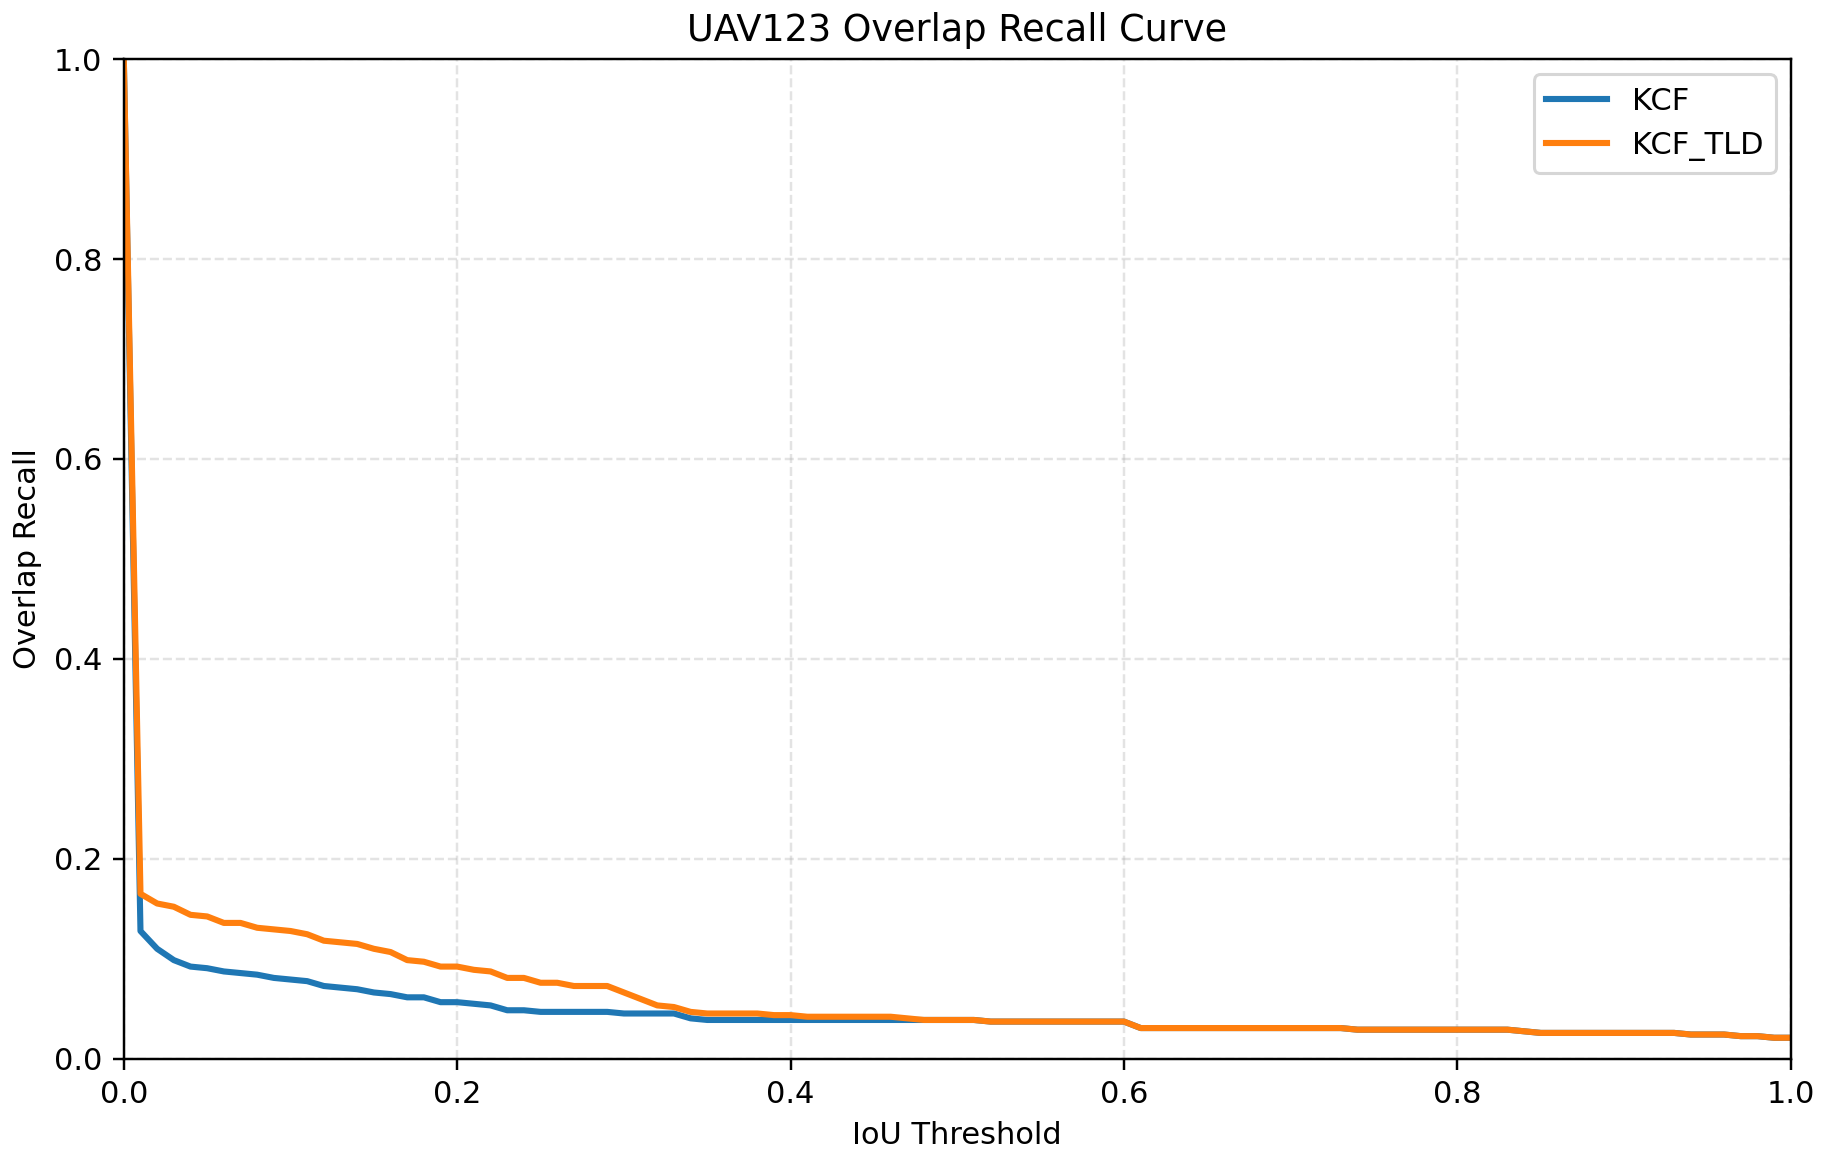
\includegraphics[width=\textwidth]{result_overlap_curve_cropped.png}
		\caption{Overlap recall curve}
	\end{subfigure}
	\hfill
	\begin{subfigure}[t]{0.48\textwidth}
		\centering
		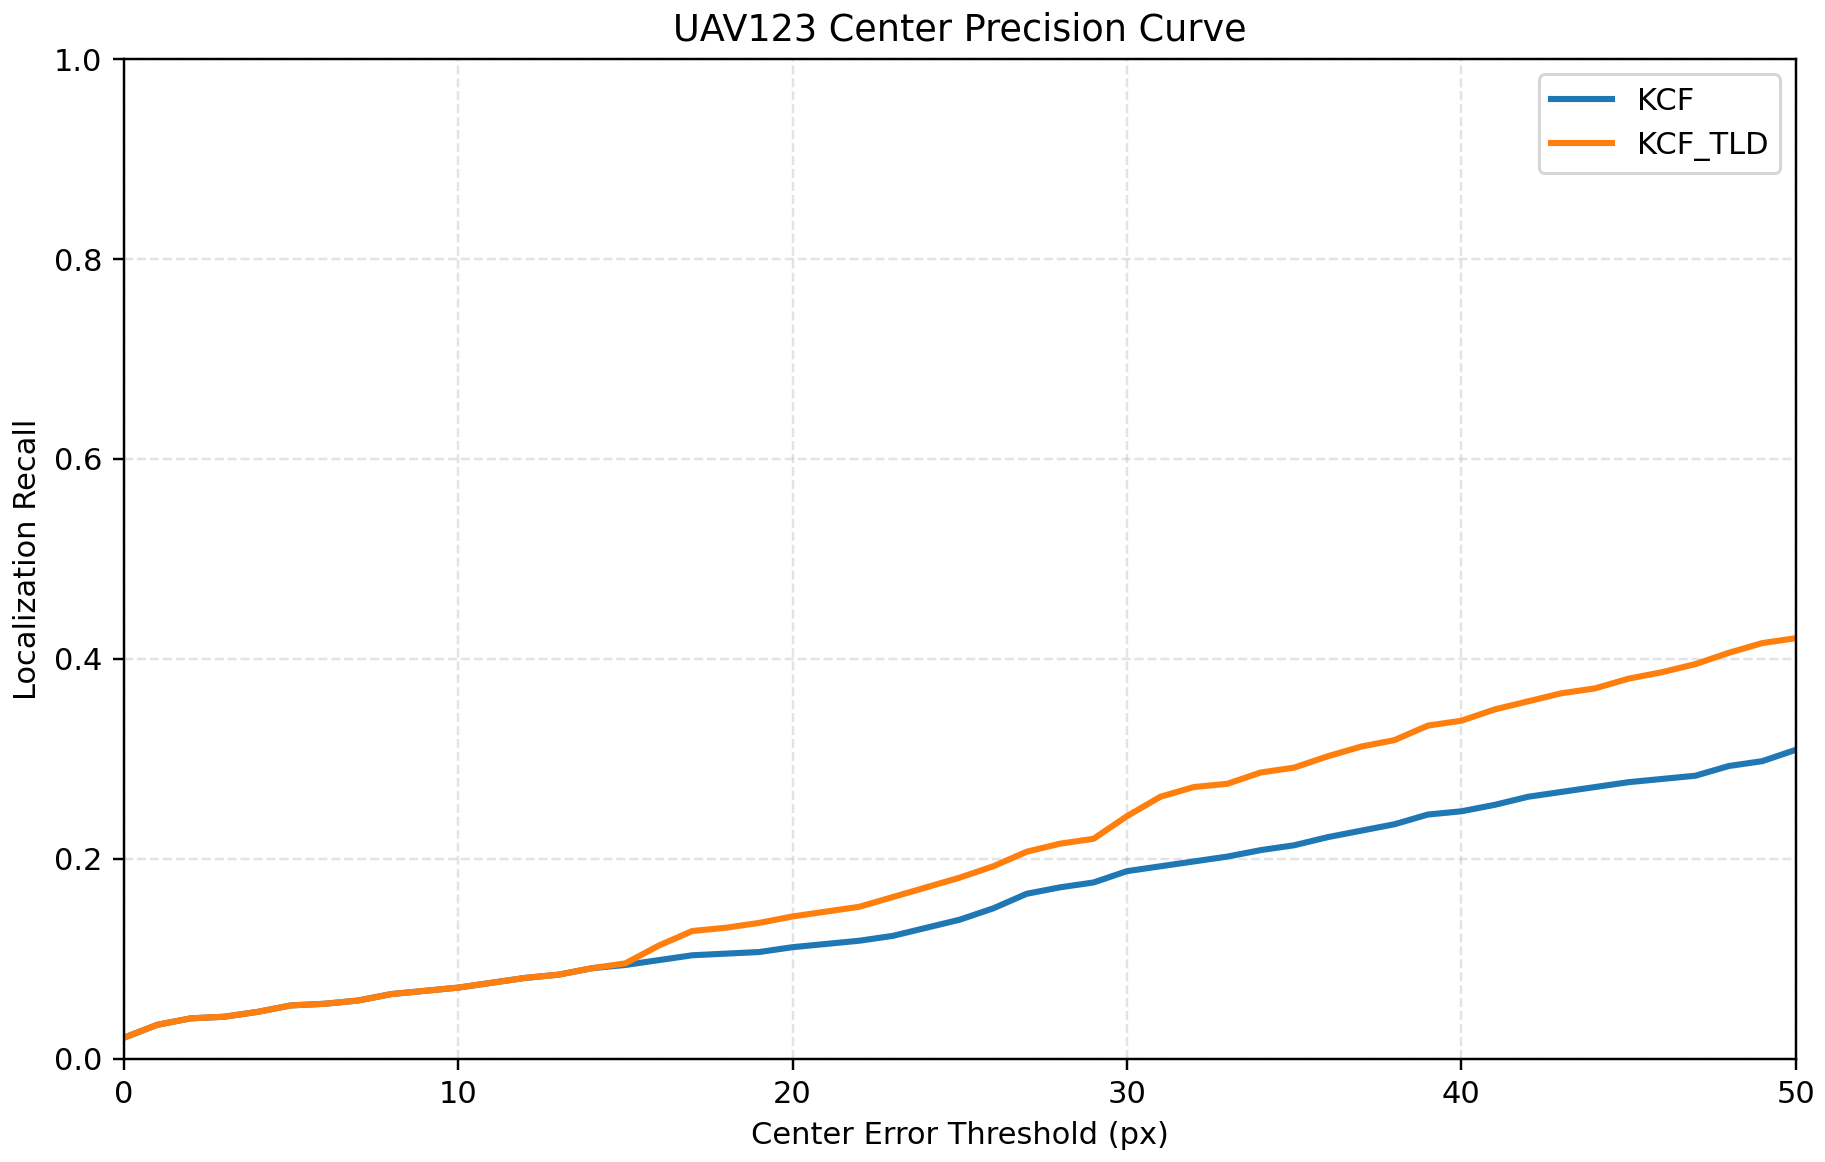
\includegraphics[width=\textwidth]{result_center_precision_curve_cropped.png}
		\caption{Center precision curve}
	\end{subfigure}
	\caption{Paired benchmark curves for the current KCF versus KCF\textendash TLD comparison.}
	\label{fig:curves-paired}
\end{figure}

\begin{figure}[htbp]
	\centering
	\begin{subfigure}[t]{0.48\textwidth}
		\centering
		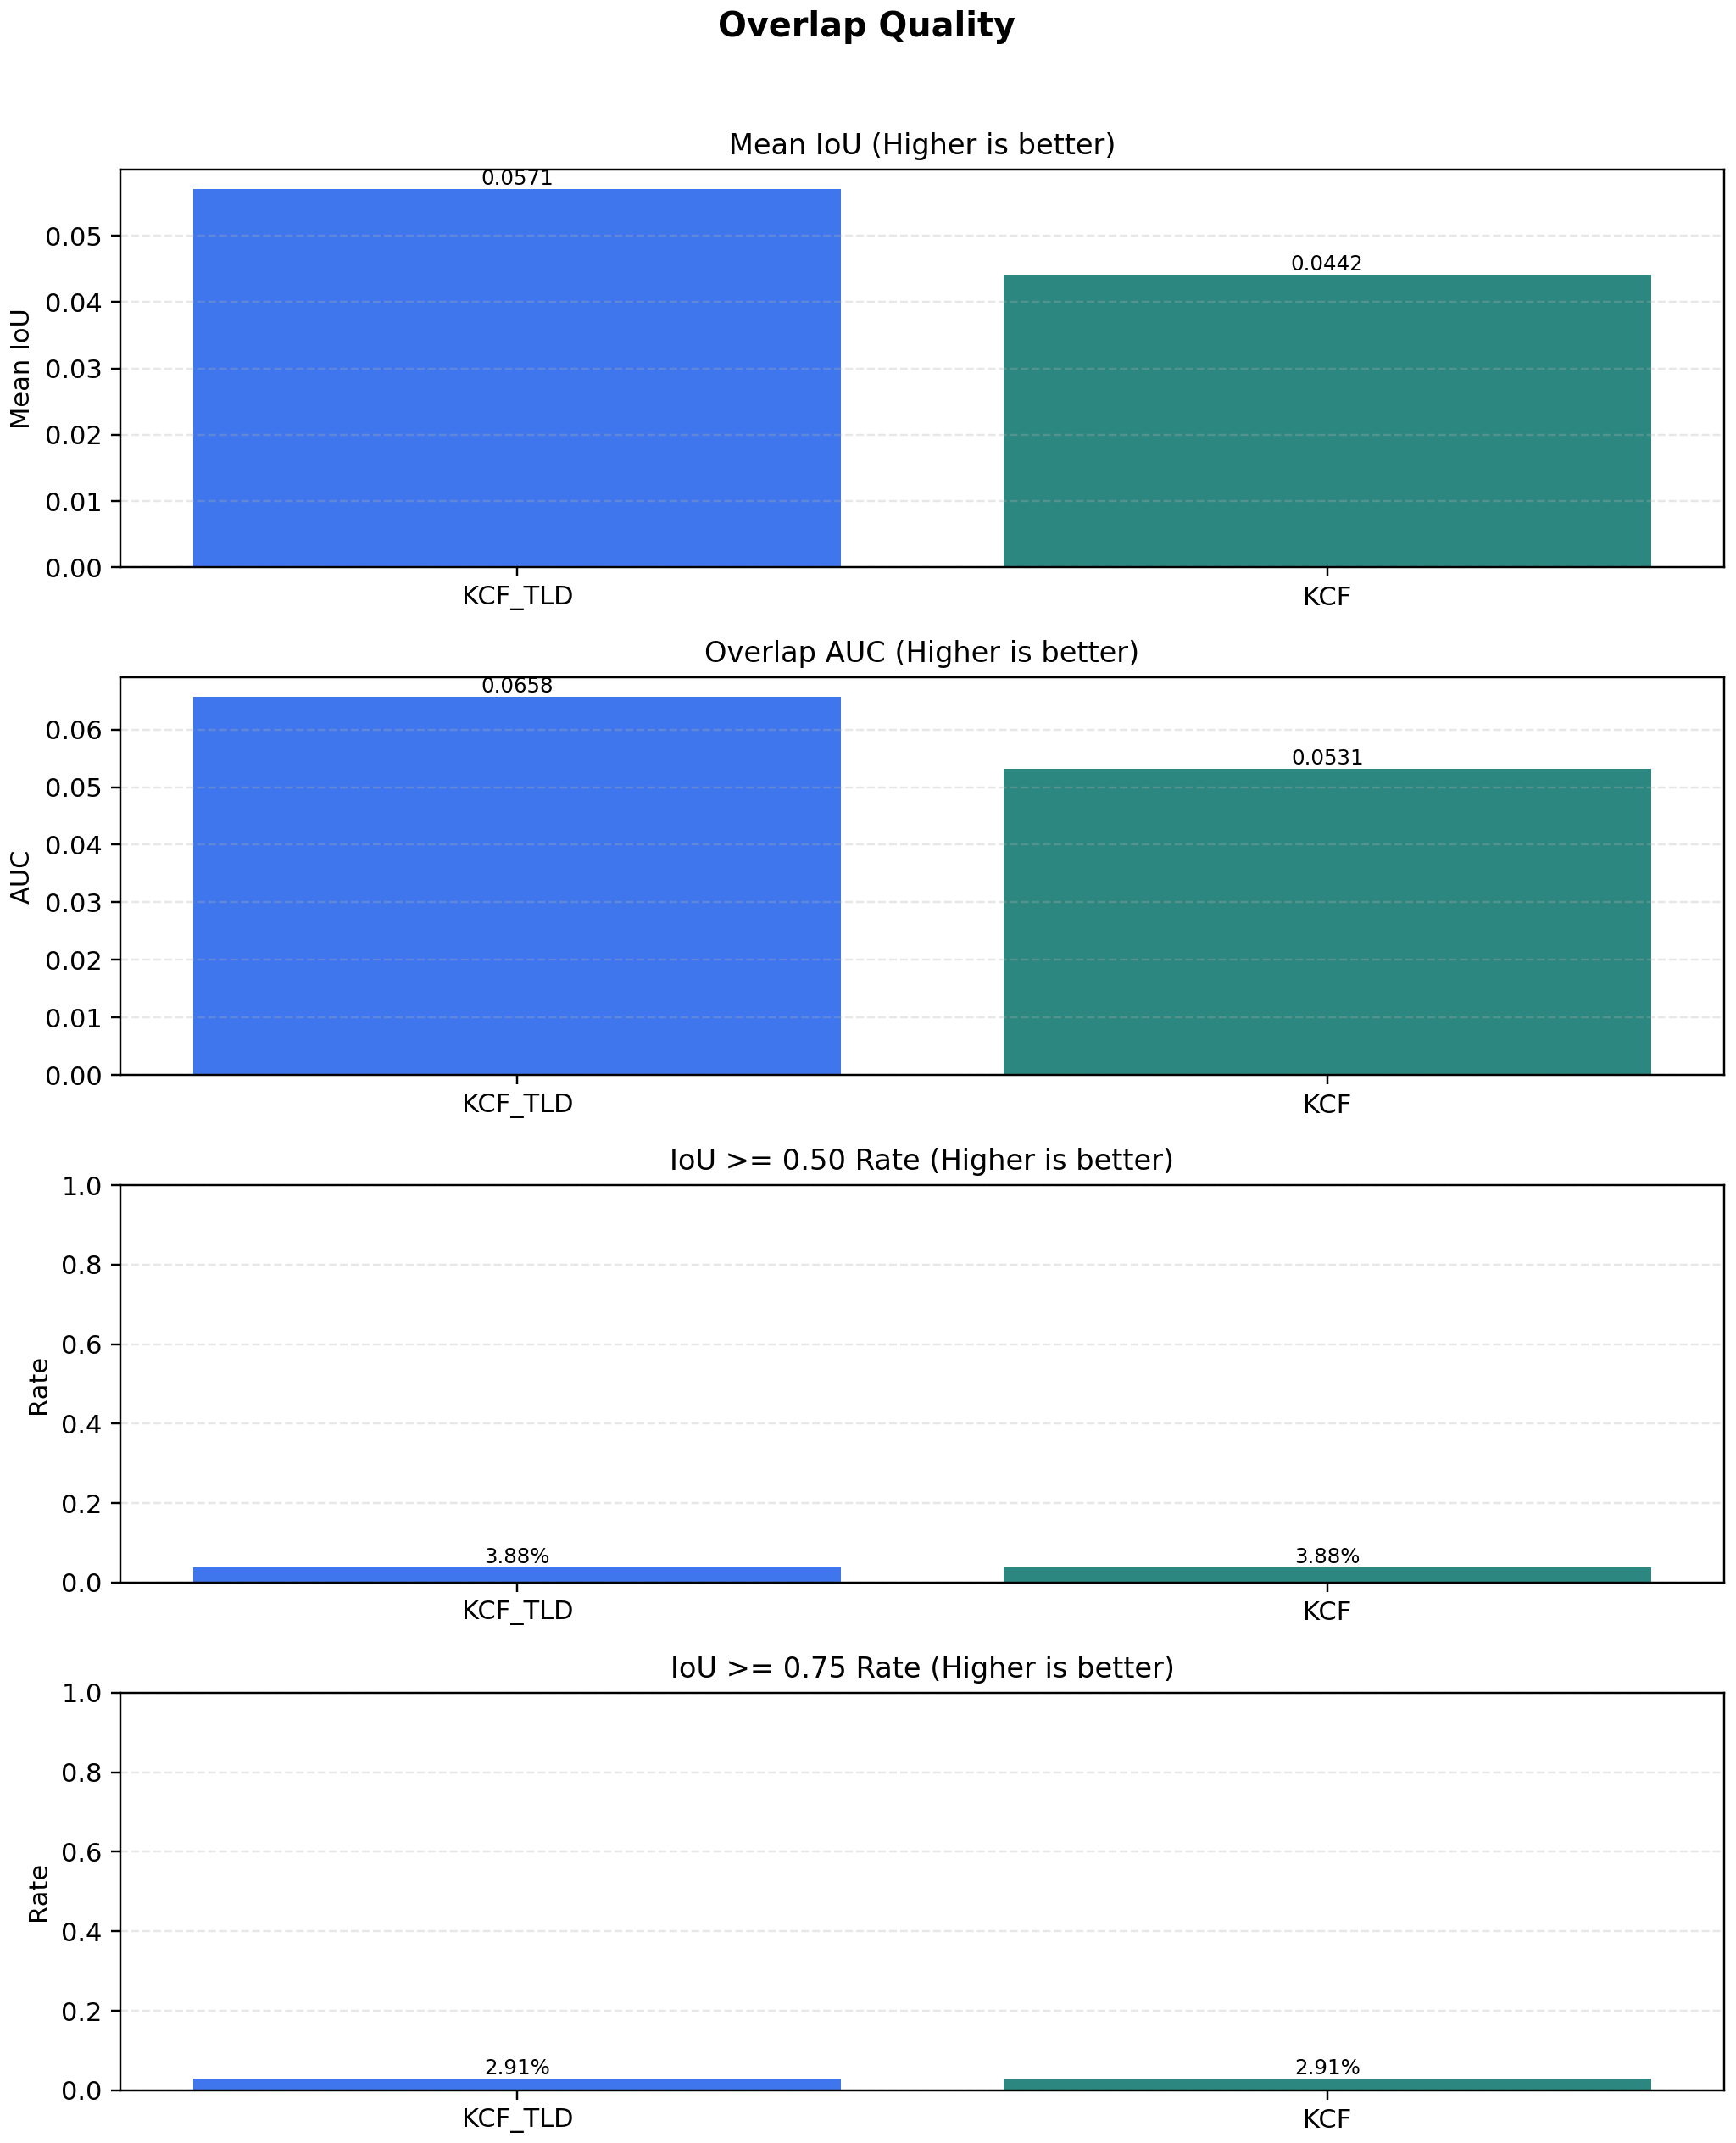
\includegraphics[width=\textwidth]{result_overlap_metrics_cropped.png}
		\caption{Overlap quality metrics}
	\end{subfigure}
	\hfill
	\begin{subfigure}[t]{0.48\textwidth}
		\centering
		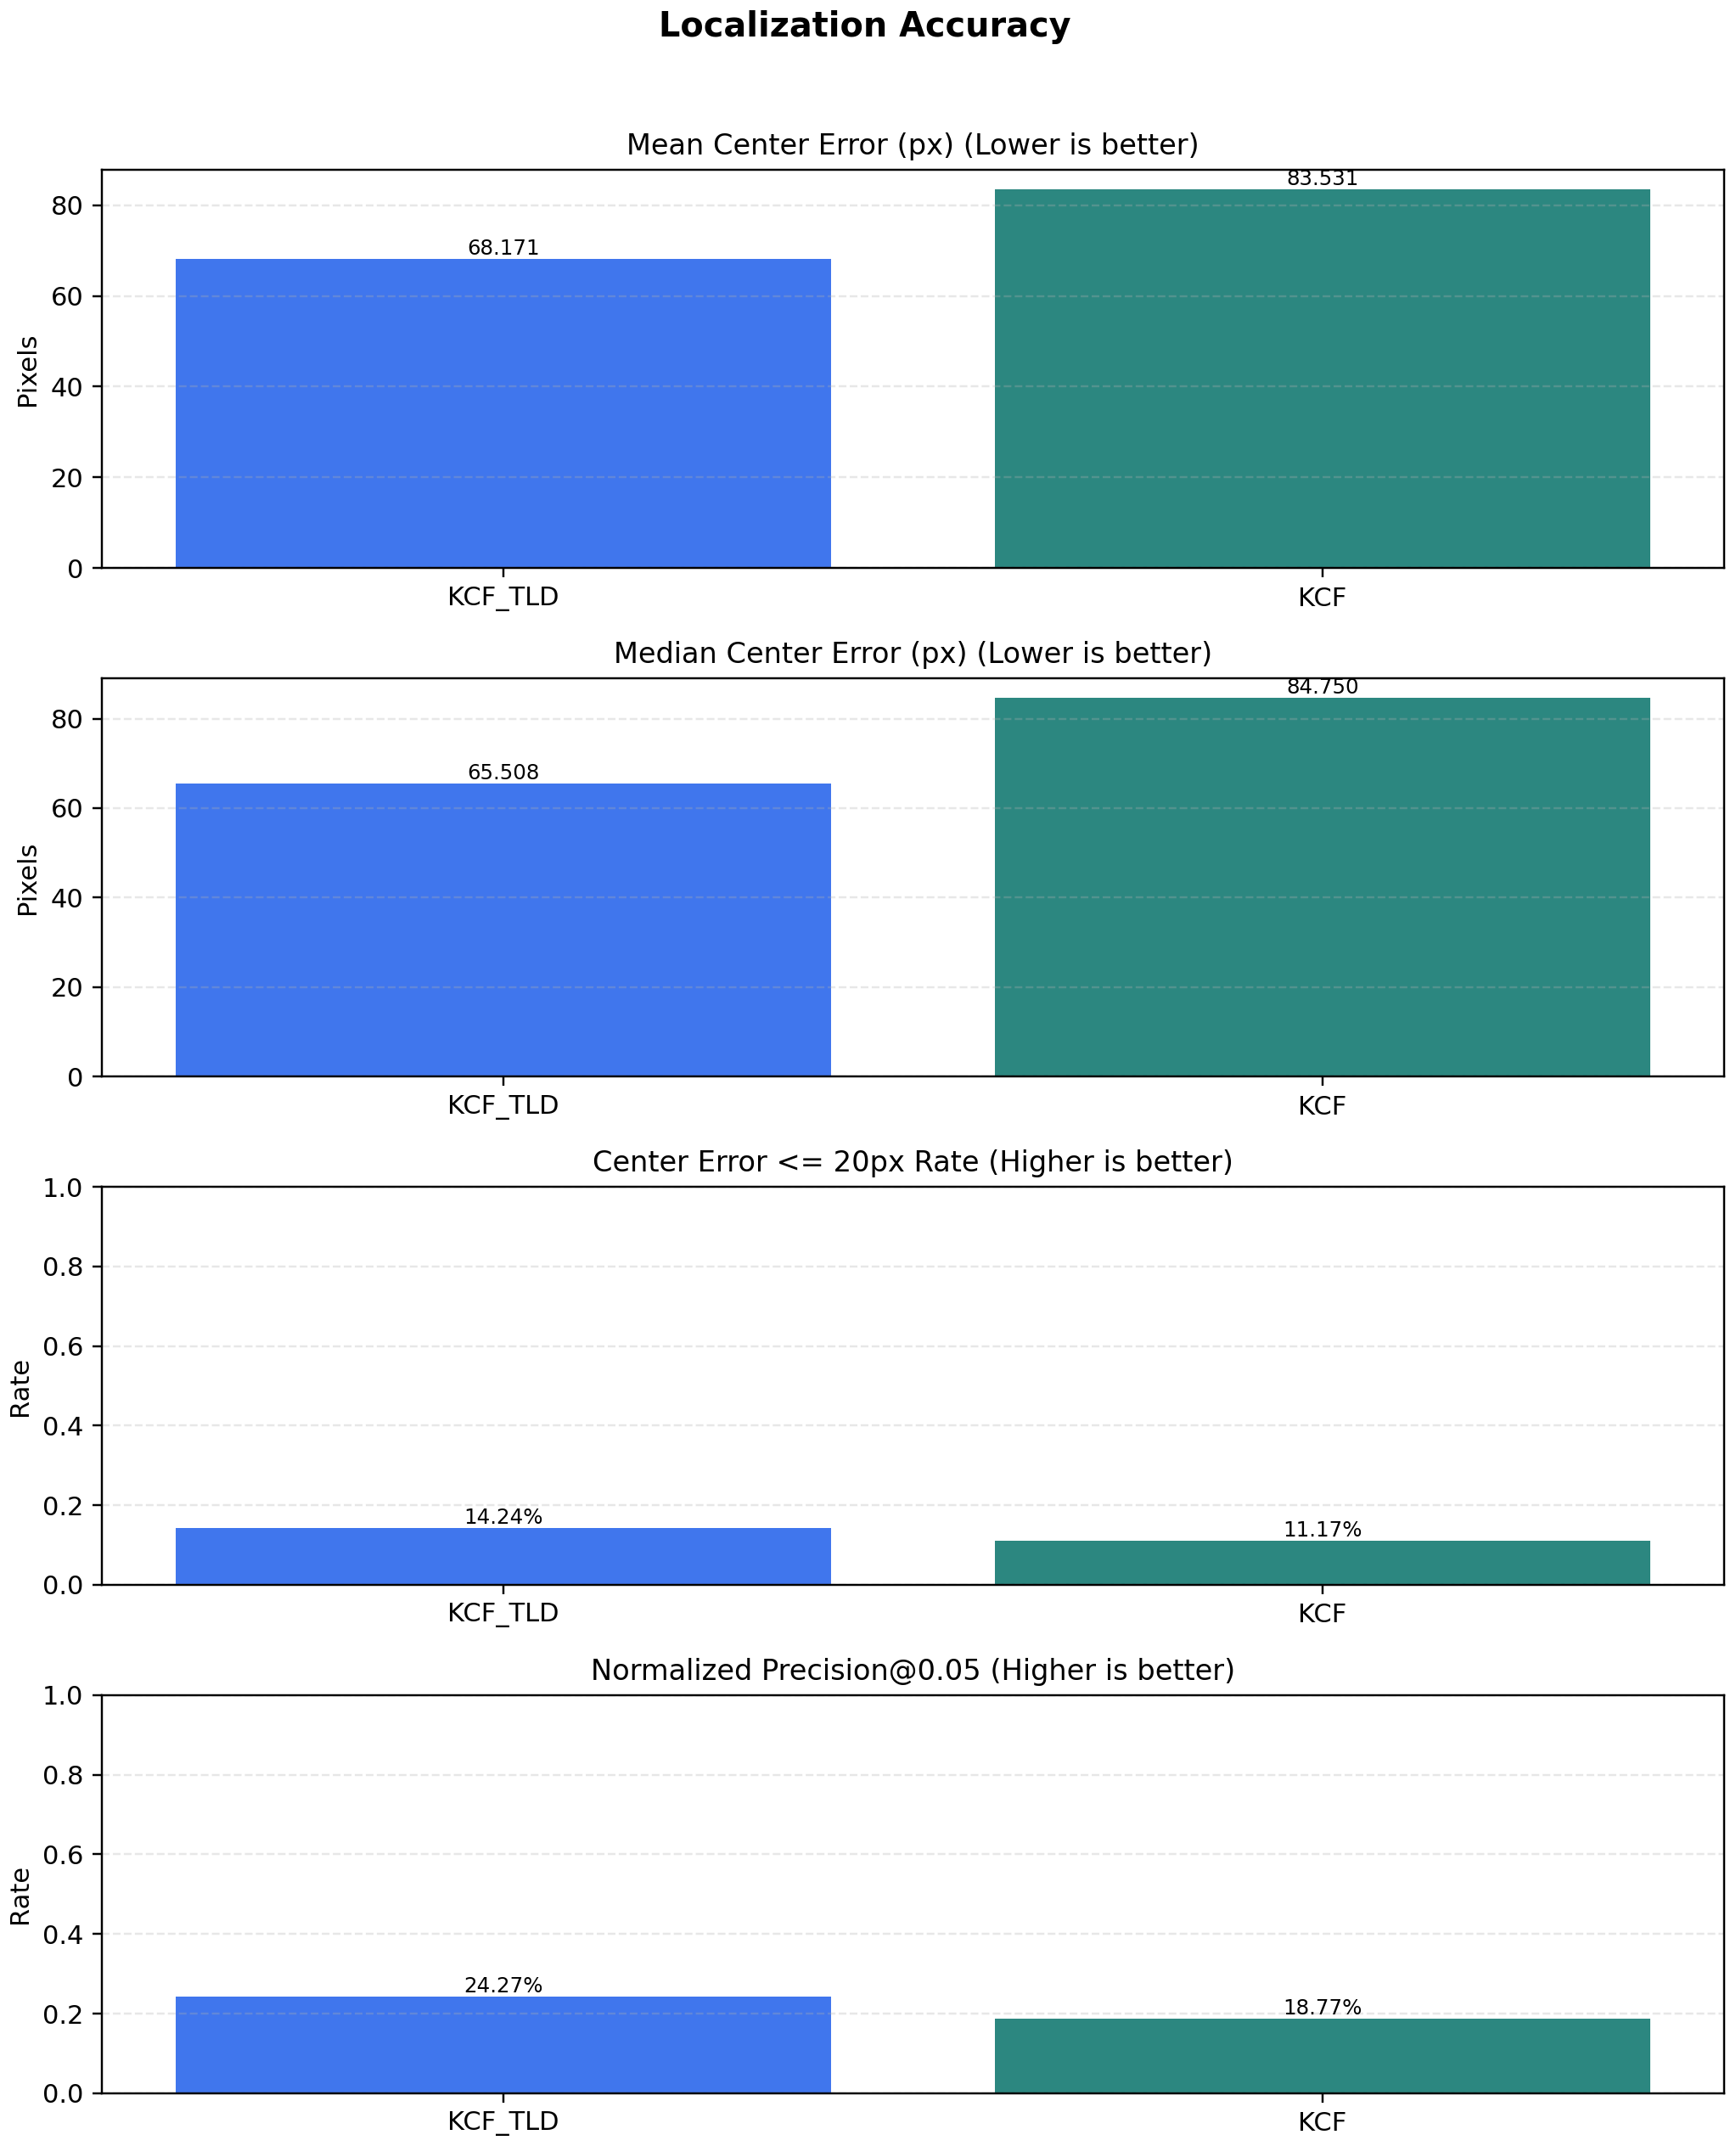
\includegraphics[width=\textwidth]{result_localization_metrics_cropped.png}
		\caption{Localization accuracy metrics}
	\end{subfigure}

	\vspace{0.8em}

	\begin{subfigure}[t]{0.48\textwidth}
		\centering
		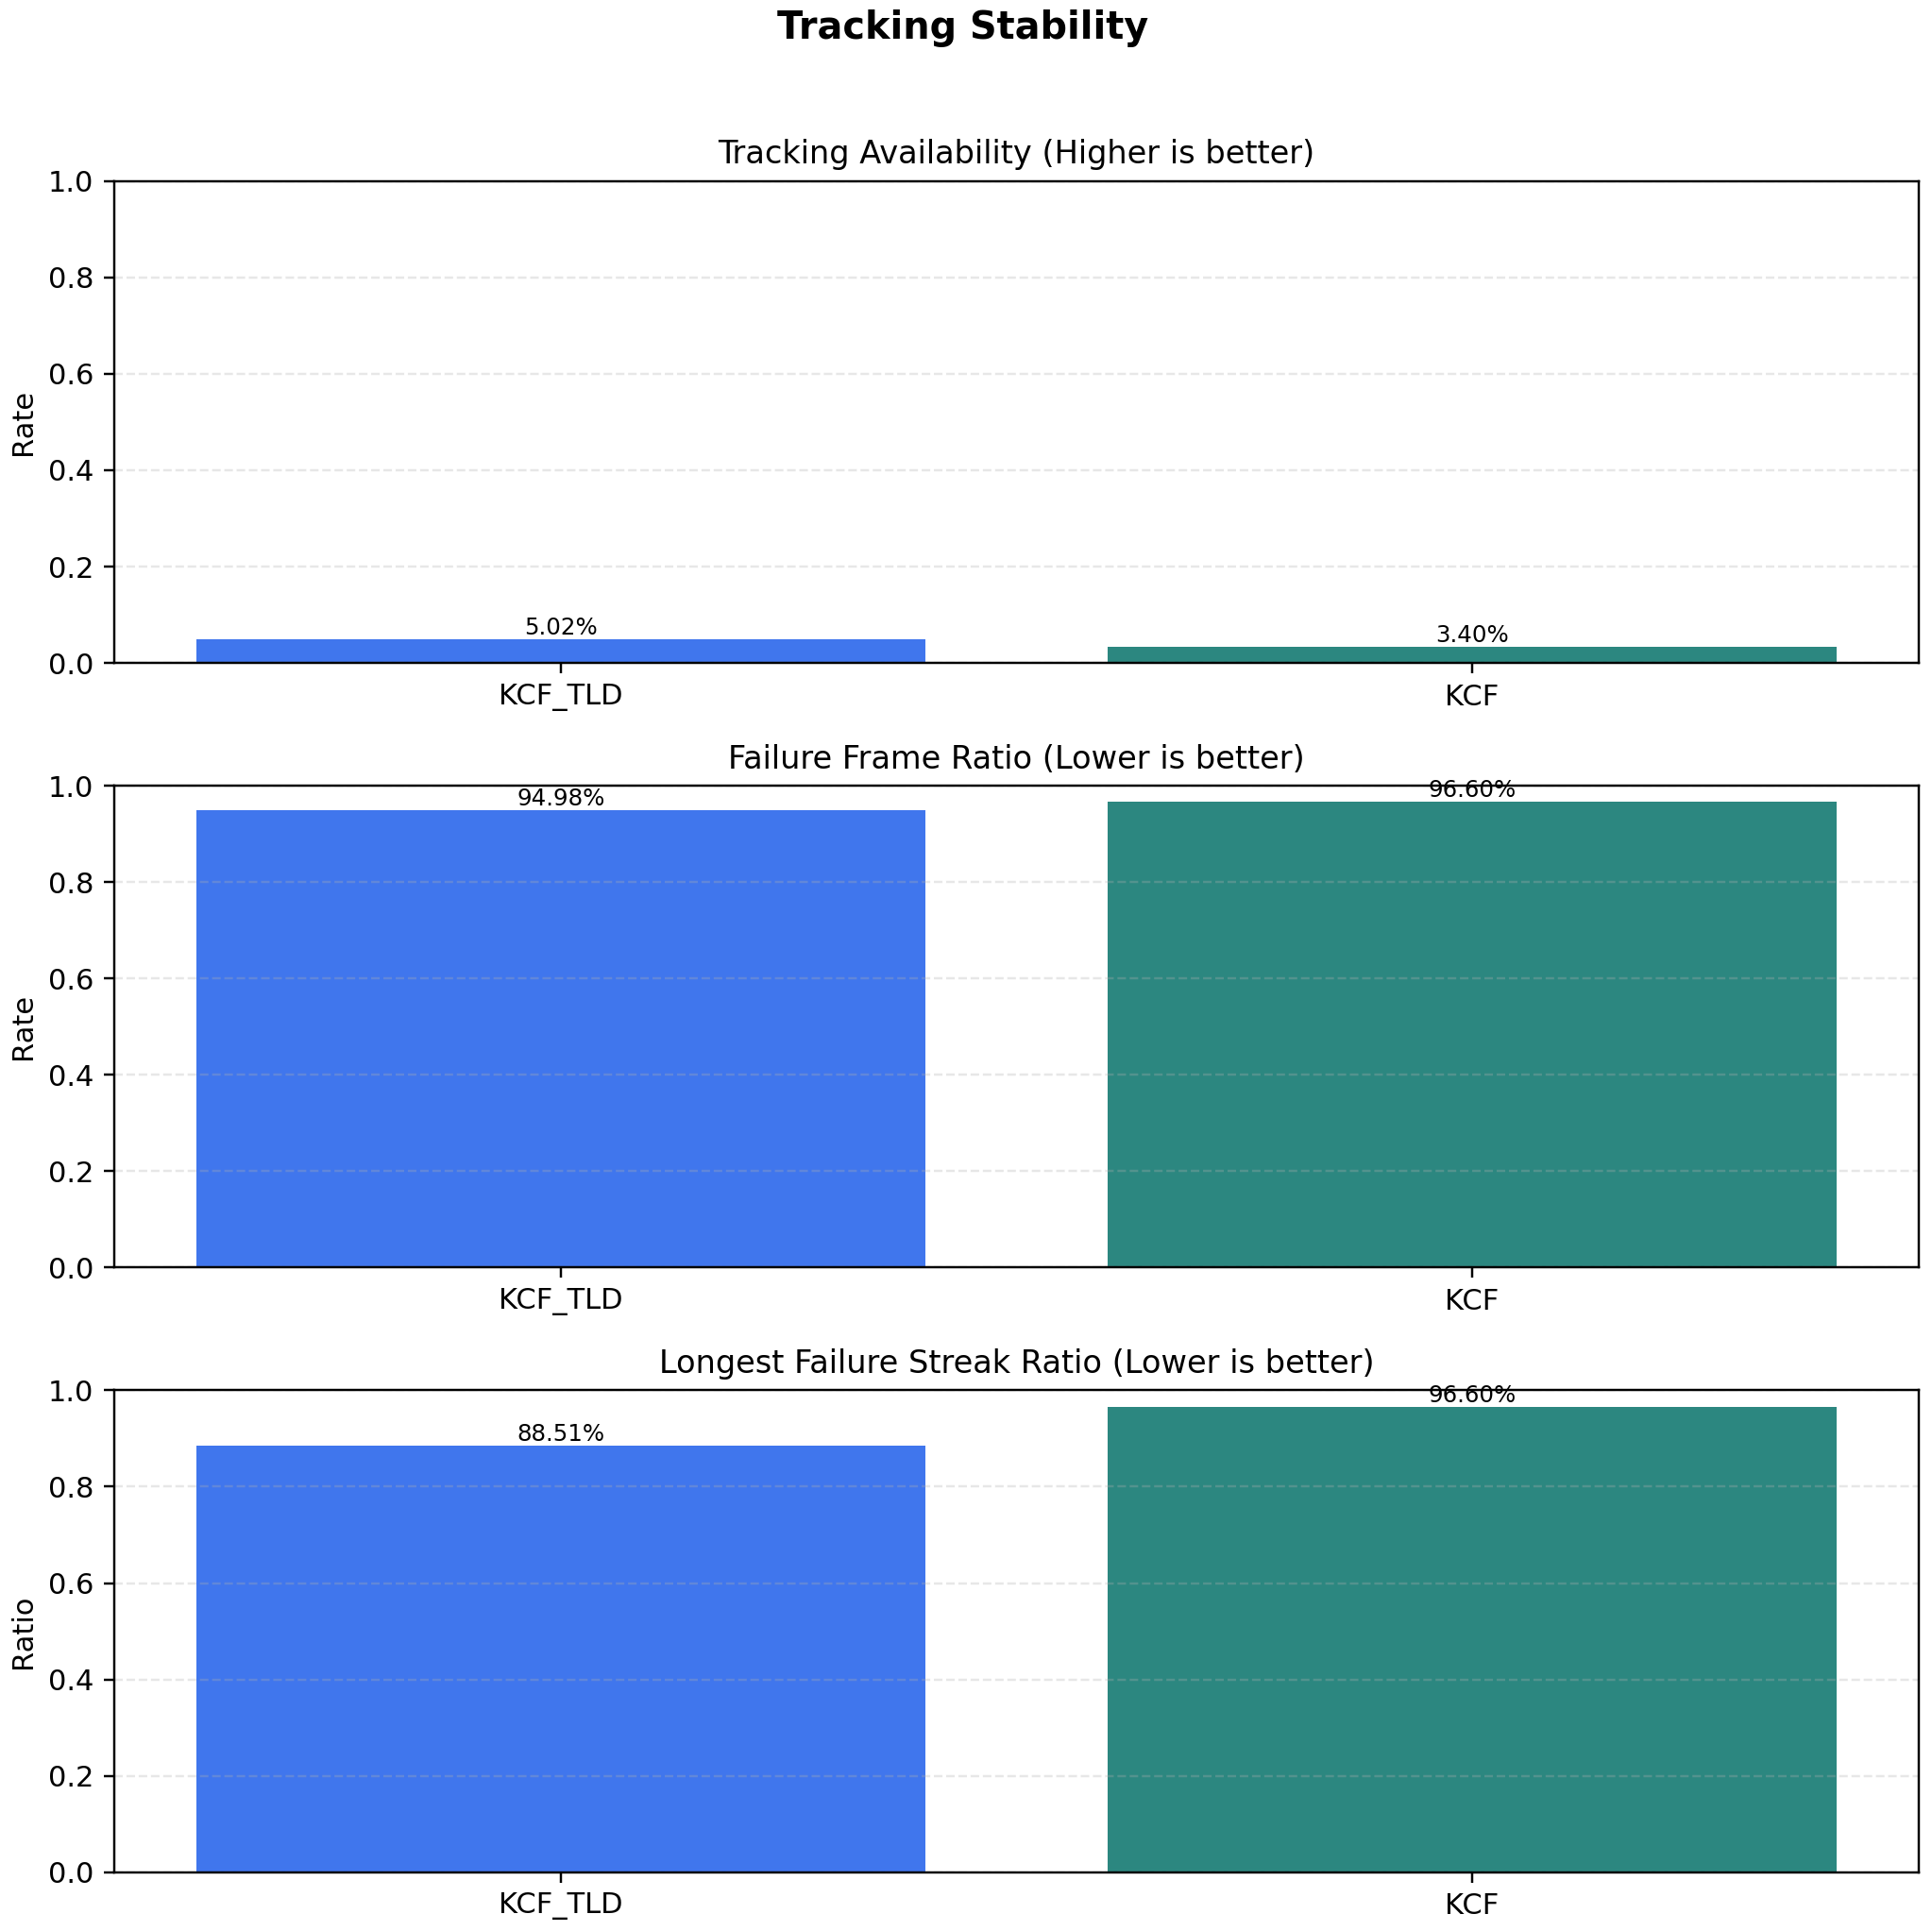
\includegraphics[width=\textwidth]{result_stability_metrics_cropped.png}
		\caption{Tracking stability metrics}
	\end{subfigure}
	\hfill
	\begin{subfigure}[t]{0.48\textwidth}
		\centering
		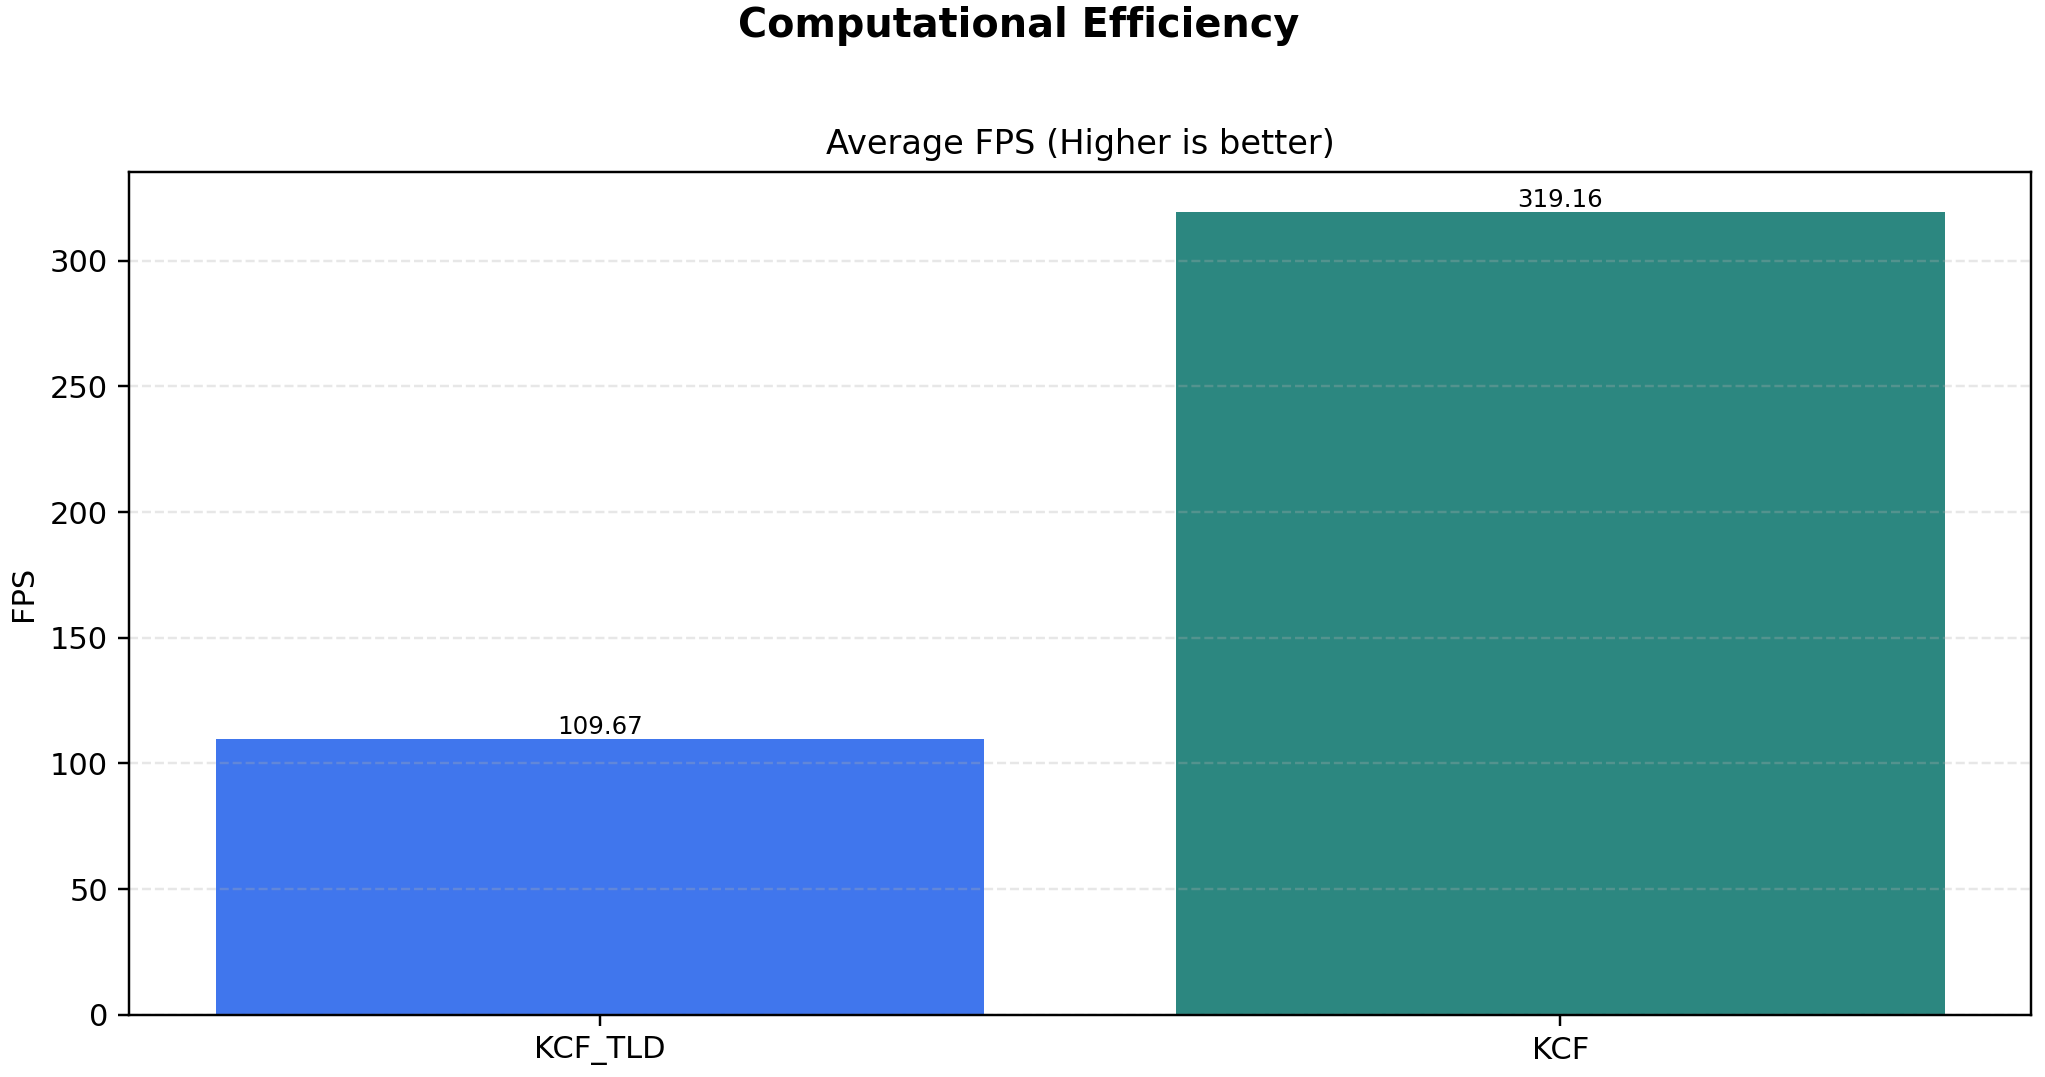
\includegraphics[width=\textwidth]{result_efficiency_metrics_cropped.png}
		\caption{Computational efficiency metrics}
	\end{subfigure}
	\caption{Grouped benchmark metrics in a two-row layout. These panels correspond to the four evaluation categories used in the benchmark pipeline.}
	\label{fig:metrics-grid}
\end{figure}

\begin{figure}[htbp]
	\centering
	\begin{subfigure}[t]{0.48\textwidth}
		\centering
		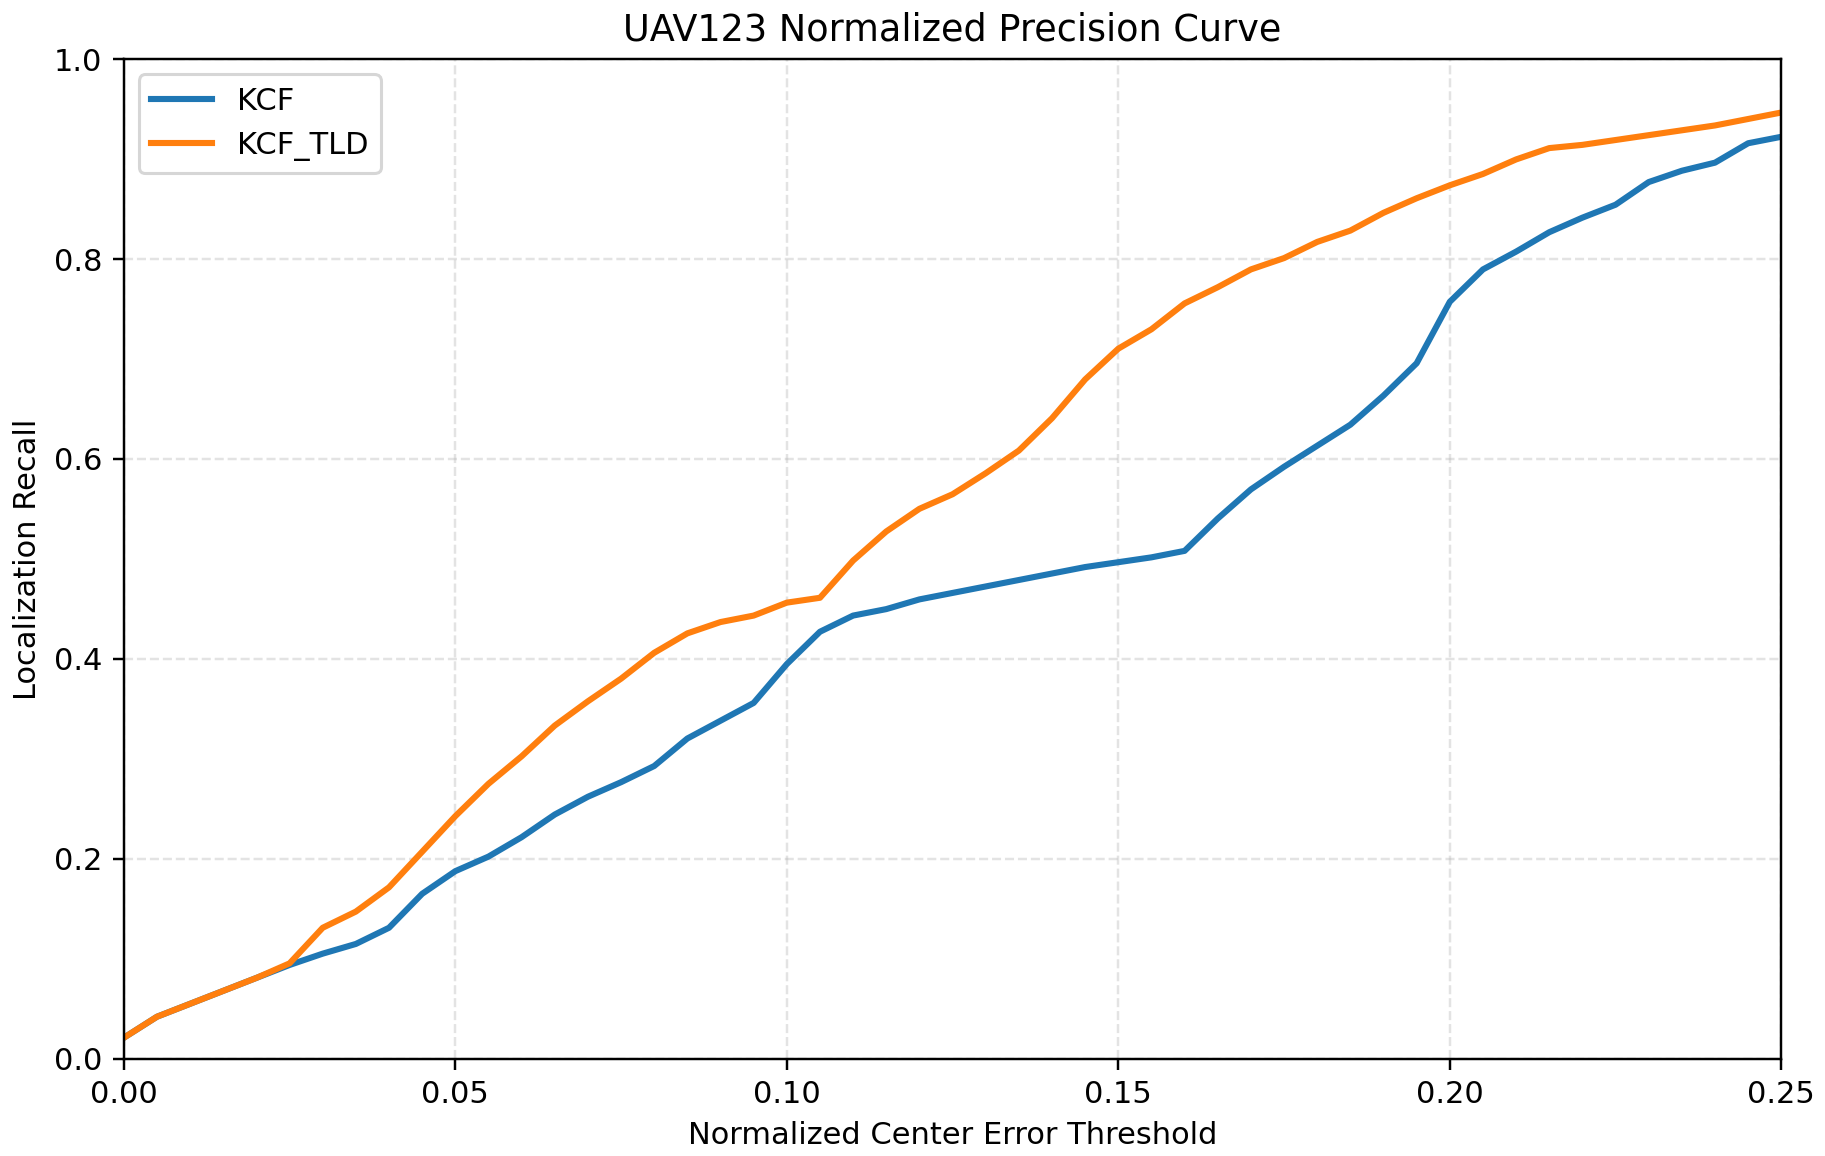
\includegraphics[width=\textwidth]{result_normalized_precision_curve_cropped.png}
		\caption{Normalized precision curve}
	\end{subfigure}
	\hfill
	\begin{subfigure}[t]{0.48\textwidth}
		\centering
		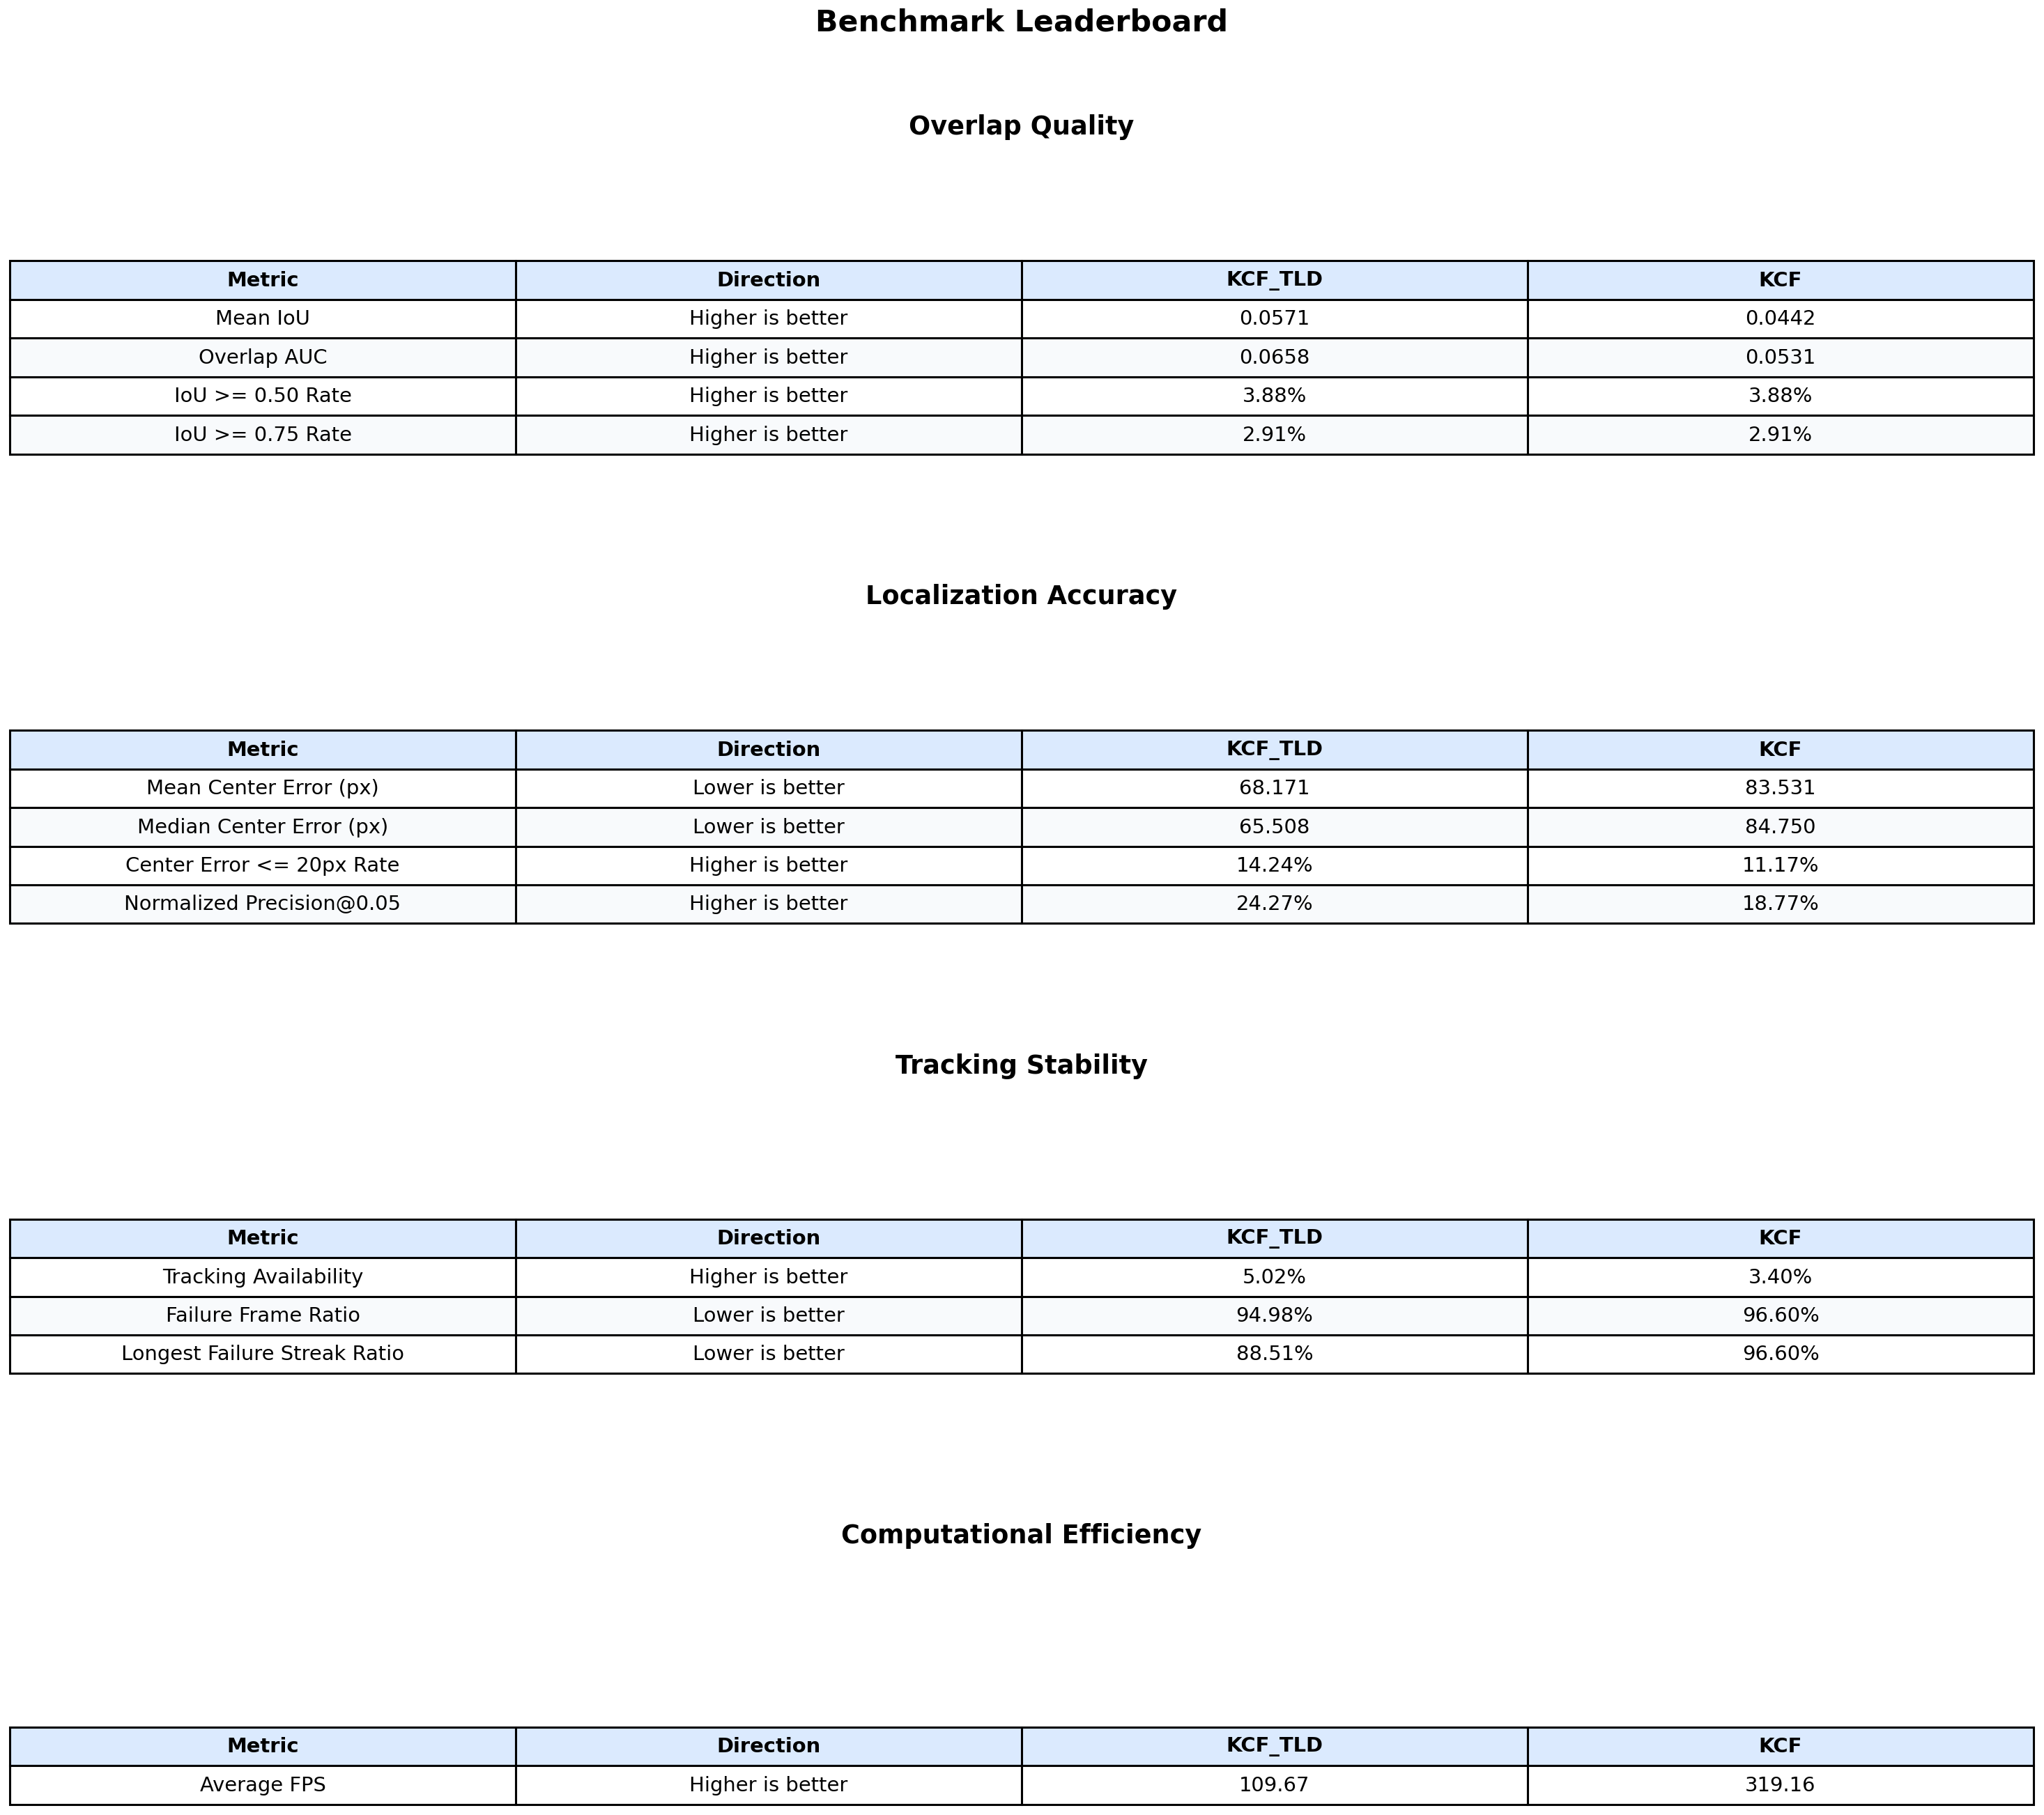
\includegraphics[width=\textwidth]{result_leaderboard_cropped.png}
		\caption{Benchmark leaderboard}
	\end{subfigure}
	\caption{Additional benchmark outputs showing normalized precision and the aggregate leaderboard.}
	\label{fig:norm-leaderboard}
\end{figure}

\section{Discussion}
At the same time, the current method still has several important limitations. The first is structural: since the normal stage is still dominated by KCF, the system's upper bound remains strongly constrained by KCF itself. If KCF drifts in a way that isn't fully captured by the heuristic reliability tests, the recovery branch may still be activated too late --- or it may be activated using an already degraded reference box. The second limitation is the trigger logic. It relies on hand-crafted geometric thresholds, which are easy to implement but may not distinguish harmless short-term fluctuation from genuine failure in complex UAV scenes. The third limitation is efficiency. The latest profiling results show that the major slowdown in difficult sequences is caused by the TLD branch itself rather than by the KCF path or by state switching overhead. So, simply adjusting thresholds won't fundamentally solve the efficiency problem.

The experimental evidence still supports a clear interpretation of the algorithms discussed here. KCF remains attractive because its computational pathway is simple and well suited to short-term local tracking. CSRT extends the same family of ideas and usually gives better box quality plus stronger robustness, but at a heavier computational cost. TLD contributes something different --- not necessarily better frame-by-frame localisation, but a stronger conceptual answer to long-term failure. Interestingly, that's exactly why TLD is better treated as a recovery-oriented component than as a permanently active high-speed tracker.

The proposed KCF\textendash TLD method inherits both the strengths and the weaknesses of that division of labour. Its strengths are fairly clear, though not perfectly balanced. First, the system logic is easy to interpret: KCF handles fast tracking, while TLD is reserved for recovery. Second, the method adds explicit protection against erroneous recovery through several gates --- activation thresholds, geometric continuity tests, consistency checks, and a lightweight plausibility filter. Third, the implementation is clearly aware of efficiency, since interval control and recovery timeout stop the system from remaining in a permanently slow state.

These observations also suggest the most reasonable future directions. One direction is to improve the trigger mechanism by combining motion continuity, short-term response stability, and trajectory history so that the system can decide more intelligently when recovery is truly needed. Another direction is to improve recovery validation through higher-level information. Instead of relying only on overlap and scale consistency, future work could use stronger appearance cues, temporal trend modelling, or multimodal reasoning to judge whether a candidate is really compatible with recent target behaviour. If those mechanisms are introduced carefully, the hybrid design could become more adaptive without losing interpretability.

\section{Conclusion}
This paper has presented an English analysis of three classical discriminative UAV trackers: KCF, CSRT, and TLD. It has also introduced a hybrid KCF\textendash TLD relocalization strategy. The comparison shows that the three methods differ not only in implementation detail, but also in tracking philosophy. KCF prioritises speed. CSRT prioritises robustness through reliability modelling. TLD prioritises long-term recovery through explicit detection and online learning. All in all, these differences explain why no single classical tracker can simultaneously optimise real-time throughput, localisation quality, and failure recovery.

To address that gap, the proposed KCF\textendash TLD method assigns different responsibilities to two complementary trackers. KCF is used during the normal stage to preserve high-speed tracking, while TLD is triggered only after KCF becomes unreliable or loses the target. The method then applies interval control, timeout protection, overlap constraints, consistency confirmation, and plausibility filtering before accepting a recovery. In the current benchmark subset, this design improves KCF in average IoU, overlap AUC, centre precision, and tracking availability, which confirms that the role-based combination is meaningful. But the experiments also show a major practical limitation: the TLD recovery branch can impose severe runtime overhead on difficult sequences, so the current system can't yet preserve KCF's raw FPS advantage.

Overall, the proposed method verifies the feasibility of the ``high-speed main tracker plus auxiliary recovery module'' idea, but it should still be seen as an intermediate design rather than a fully mature final solution. Future work should focus on more intelligent recovery triggering, more adaptive validation of recovery candidates, and more efficient long-term relocalization modules. Surprisingly, the present results make that future path clearer rather than less clear, because they show exactly where the system still breaks down.

\printbibliography[title={References}]

\end{document}